\documentclass[12pt,a4paper,titlepage]{article}
\usepackage[italian]{babel}
\usepackage[T1]{fontenc}
\usepackage[latin1]{inputenc}
\usepackage{titlesec}
\usepackage[hidelinks]{hyperref}
\usepackage[a4paper,top=2cm,bottom=2cm,left=1cm,right=1cm]{geometry}
\usepackage{soulutf8,color}
\usepackage{emptypage}                     
\usepackage{fancyhdr}
\usepackage{graphicx}
\usepackage{float}
\pagestyle{fancy}

\begin{document}

\title{ANALISI DEI REQUISITI}
\author{SWEg Group}
\date{}
\maketitle

\lhead{SWEg Group}
\chead{}
\lfoot{Analisi dei Requisiti}
\cfoot{}
\rfoot{\thepage}
\renewcommand{\headrulewidth}{0.2pt}
\renewcommand{\footrulewidth}{0.2pt}
\rhead{Registro Modifiche}
\section{Registro Modifiche}
\small %rippicciolisce il testo

{\renewcommand\arraystretch{1.2}  %aumenta l'altezza di ogni riga
\begin{tabular}{|l|c|c|c|}
	\hline
	{\textbf{Modifica}}&{\textbf{Nome}}&{\textbf{Data}}&{\textbf{Ver.}}\\
	\hline
	Creazione Raw Documento & Gianluca Crivellaro & 21/12/2016 & 0.0.1 \\
	\hline
	Modifica Raw & Gianluca Crivellaro & 22/12/2016 & 0.0.2 \\
	\hline
	Aggiunti Requisiti & Sebastiano Marchesini & 23/12/2016 & 0.0.3 \\
	\hline
	Aggiunti Requisiti Estesi Concordati & Gianluca Crivellaro & 27/12/2016 & 0.0.4 \\
	\hline
	Stesura Documento (Introduzione) & Sebastiano Marchesini &  28/12/2016 & 0.1.0 \\
	\hline
	Creazione Grafici UML & Pietro Lonardi e Gianluca C. & 29/12/2016 & 0.1.1 \\
	\hline
	Stesura Documento (Descrizione Generale \& Casi d'Uso) & Sebastiano Marchesini & 30/12/2016 & 0.1.2 \\
	\hline
	Creazione Grafici UML & Pietro Lonardi & 02/01/2017 & 0.1.3 \\
	\hline
	Verifica Documento \& Grafici UML & Piergiorgio Danieli & 03/01/2017 & 0.1.4 \\
	
	\hline
\end{tabular}
}	\normalsize
\newpage

\tableofcontents
\thispagestyle{empty}

\newpage



\rhead{Introduzione}
\section{Introduzione}
\subsection{Scopo del Documento}
Tale documento ha lo scopo di studiare e modellare concettualmente il problema che si pone con APIM. Posizionando le componeti (o ambiti) a scopo di allocazione dei requisiti. Alcuni dei requisiti specificandoli con il diagramma dei casi d'uso.

Vi deve essere la certezza di non aver lasciato dimenticato nessuno tra i bisogno espliciti e i bisogni impliciti. Questo implica che non vi sia ambiguità tra i requisiti.
Bisogna sempre tener conto di portare al massimo possibile la granularità del problema, senza però confonderlo e renderlo impossibile da verificare. Questo per rendere il requisito decidibile.

È infine bene tener presente otto semplici qualità di selezione dei requisiti:
\begin{itemize}
\item Non Ambigui
\item Corretti
\item Completi
\item Verificabili
\item Consistenti
\item Modificabili
\item Tracciabili
\item Ordinati per Rilevanza
\end{itemize}
\subsection{Scopo del Prodotto}
L'obbiettivo è creare un'infrastruttura che permetta la distribuzione digitale e la gestione dei diritti digitali di microservizi. Creati e importati da diversi utenti che possono interfacciarsi tra loro.

Viene usata per gestire e distribuire una vasta gamma di microservizi (alcuni esclusivi) e il loro relativo supporto. Tutte queste operazioni sono effettuate via Internet.
È inoltre possibile il monitoraggio di ogni API grazie alle tecnologie fornite dal prodotto. 
\subsection{Glossario}
Alla fine di evitare ambiguità e mantenere la consistenza il Glossario è un documento unico e consultabile separatamente. \\
Un glossario è una raccolta di termini di un ambito specifico e circoscritto. In questo caso per raccogliere termini desueti e specialistici inerenti al progetto. 
\\
\subsection{Riferimenti}
\subsubsection{Normativi}
\begin{itemize}
\item \textbf{Norme di Progetto}:	"Norme di Progetto v1.0.0".
\item \textbf{Capitolato d'appalto C1}:	API Market per microservizi \\
\textcolor{blue}{\url{www.math.unipd.it/~tullio/IS-1/2016/Progetto/C1.pdf}}. 
\item \textbf{Verbali}:
\subsubsection{Informativi}
\item \textbf {Studio di Fattibilità}: "Studio di Fattibilità v.1.0.0".
\item \textbf{IEEE 830-1998}: Recommended Practice for Software Requirements Specifica- tions \\
\textcolor{blue}{\url{https://en.wikipedia.org/wiki/Software_requirements_specification}}.
\end{itemize}

\newpage

\rhead{Descrizione Generale}
\section{Descrizione Generale}
\subsection{Obbiettivi del prodotto}
L'obbiettivo primario del prodotto é di dare ad ogni utente la possibilità di registrare il proprio microservizio in una piattaforma dedicata. In questo modo è possibile la vendita (o condivisione) con gli altri utenti della comunità regolata da politiche di compravendita specifiche e flessibili a seconda dello scopo dell'API o del volere del tecnico. 

L'obbiettivo è quindi quello di incentivare la programmazione a microservizi e, oltre a spingere i gruppi più piccoli nel progettare per il mercato virtuale, pensare sempre di più a delle migliori architetture flessibili invece che veri e propri programmi. Si vuole abbandonare i vecchi programmi monolite per entrare in una realtà fatta di sistemi divisi in moduli, la nuova sfida progettuale sarà quindi unire i vari microservizi (o API) per costruire un prodotto completo.
\subsection{Funzioni del prodotto}
SWEg Group si impegna in particolar modo alle sottoscritte funzioni del prodotto :
\begin{enumerate}
\item \textbf{Registrare le API di un microservizio}:	dando la possibilità di caricare un interfaccia e documentando la propria progettazione.
\item \textbf{Permetta di consultare le API}:	con un sistema di ricerca designato e filtrato anche con dati tecnici . Anche se con minori funzionalità anche un utente non registrato alla piattaforma può vagliare le varie API. Per ogni api sarà inoltre possibile un consulto dei suoi dati tecnici.
\item \textbf{Permetta di associare diverse API key}: così da regolare le politiche di scambio dei microservizi. Le API key sono lo strumento principale di collegamento tra la API e il suo utilizzatore. Grazie a queste l'infrastruttura potrà regolare le scadenze , l'utilizzo e procedimento oltre ad avere un ID univoco per la monitorizzazione. 
\item \textbf{Permetta di monitorare l'utilizzo delle API}:	già accennato nei punti precedenti. Vogliamo che tale infrastruttura tenga conto di particolari dati tecnici di ogni API per renderle così misurabili in termini di efficacia ed efficienza. Oltre che a così avere un sistema automatizzato per il confronto tra i vari microservizi.
\item \textbf{Blocchi le chiamate di utenti in possesso di API key scadute e/o non valide}:	è la sottolineatura di uno dei motivi di esistenza delle API key. Punto focale per la regolamentazione dello scambio è la possibilità di acquisto delle chiavi secondo tempo, mole di scambio di dati , eccetera. I dati tecnici per le policy di durata e validità saranno descritte in seguito, ma queste decideranno se è ancora attiva una chiave o meno.
\item \textbf{Permetta di visualizzare i dati tecnici d'uso delle singole API}:	dopo aver monitorato ogni singola API è possibile fare la stima e produrre un elaborato tecnico dei valori di quest'ultima. È compito dell'API Market rendere disponibile questa funzionalità. Da parte nostra vi sarà un vaglio tra le principali e caratteristiche di interesse da dover riportare. È da parte nostra desiderabile anche la possibilità di poter visualizzare direttamente il confronto dei risultati delle caratteristiche per scegliere il microservizio migliore.
\item \textbf{Permettere di gestire una moneta virtuale per la compravendita delle API}:	il metodo di acquisto principale è comunque la moneta reale. Che può trasformarsi automaticamente in moneta virtuale con un cambio di 1:1. È possibile quindi tenere un conto personale flessibile per poter reinvestire o ritirare il contante virtuale. 
\item \textbf{Permetta di confrontare i dati tecnici delle API tra loro}:	già accennato in uno dei punti precedenti. Per una migliore visione e per scegliere il microservizio più adatto ai nostri scopi vorremo una sezione specifica di confronto dei dati tecnici. Sarà nostro compito grazie al monitoraggio avere un rapporto aggiornato e reale dell'andamento dell'API.
\item \textbf{Permetta una gestione social}:	vogliamo che quindi anche gli utenti abbiamo le loro statistiche per essere valutati. Desiderabile un programma di messaggistica interno per una comunicazione diretta e veloce. Tutto è quindi classificabile, la valutazione degli utenti delle API crea delle classifiche stimolando la concorrenza e il desiderio di popolare il market di più microservizi. Vi saranno quindi graduatorie per genere grazie alle personali esperienze e ai dati tecnici da favorire l'interazione tra gli attori della piattaforma.
\end{enumerate}
\subsection{Caratteristiche degli utenti}
Il prodotto è soprattutto proiettato a degli utenti secondo noi esperti nelle tecnologie impiegate. Abbiamo all'unisono prestabilito con il proponente del capitolato che è compito dell'utente creare l'interfaccia adeguata a registrare il microservizio nel market. Questo ci assicura una minima competenza nella programmazione e quindi nell'uso di tecnologie informatiche.

Dimestichezza nell'utilizzo di browser che sia esso da smartphone o da notebook. 
\subsubsection{Tipologia di Utenti}
Saranno 3 i principali tipi di utenti che andranno a popolare i nostri casi d'uso a seconda del livello di autenticazione nella piattaforma:
\begin{itemize}
	\item \textit{Utente non Autenticato}: è un utente che può visitare i microservizi in forma anonime a senza registrazione. Sarà limitato nelle impostazioni di ricerca, non potrà accedere alla funzionalità sociali e di compravendita delle API.
	\item \textit{Utente Autenticato}: dopo essersi registrato nel data base della piattaforma l'utente autenticato ha accesso completo alle funzionalità offerte al pubblico. Può cambiare le proprie referenze, accumulare monete virtuali e avere pieno accesso alla parte sociale. 
	\item \textit{Amministratore}:l'amministratore può modificare i profili di tutti gli utenti, modificare tutti i microservizi caricati e ha accesso a una pagina sulle statistiche del sito. Ha le funzionalità più estese e si è nominati personalmente. 
\end{itemize}

 

\subsection{Piattaforma di esecuzione}
Il prodotto finale è fruibile da qualsiasi piattaforma che disponga di un browser per la navigazione web. Sarà garantito il corretto e perfetto funzionamento con il maggior numero di browser possibili. 

La parte di back end invece sarà %BOH DITEMI VOI NON SO.
 
\subsection{Vincoli generali}
Per utilizzare le funzionalità della piattaforma è obbligatorio avere una connessione internet.
%è necessario elencare i vincoli presenti sulle tecnologie richieste e sui sistemi operativi (anche browser) supportati. 
\newpage

\rhead{Casi d'uso}
\section{Caso d'uso}
L'analisi del capitolato, il dibattito tra gli Analisti e l'incontro con ItalianaSoftware ha portato alla creazione dei casi d'uso che seguono. Si è cercato anche di studiare piattaforme sociali e di scambio simili come \textit{Steam}, \textit{Google Play} e \textit{GitHub}.

Le fonti su cui si ricavano quindi i casi d'uso sono sia impliciti, derivanti dallo studio del dominio, sia espliciti, come il capitolato d'appalto.
Ogni caso d'uso ha un codice univoco gerarchico, nella forma: 
\[UC[\textit{Codice Univoco del Padre}].[\textit{Codice Progressivo di Livello}]\] 
Il codice progressivo può includere diversi livelli di gerarchia separati da un punto.
\clearpage
\subsection{Caso d'uso Generale: Operazioni ad alto livello}
\begin{figure}[ht]
	\centering
	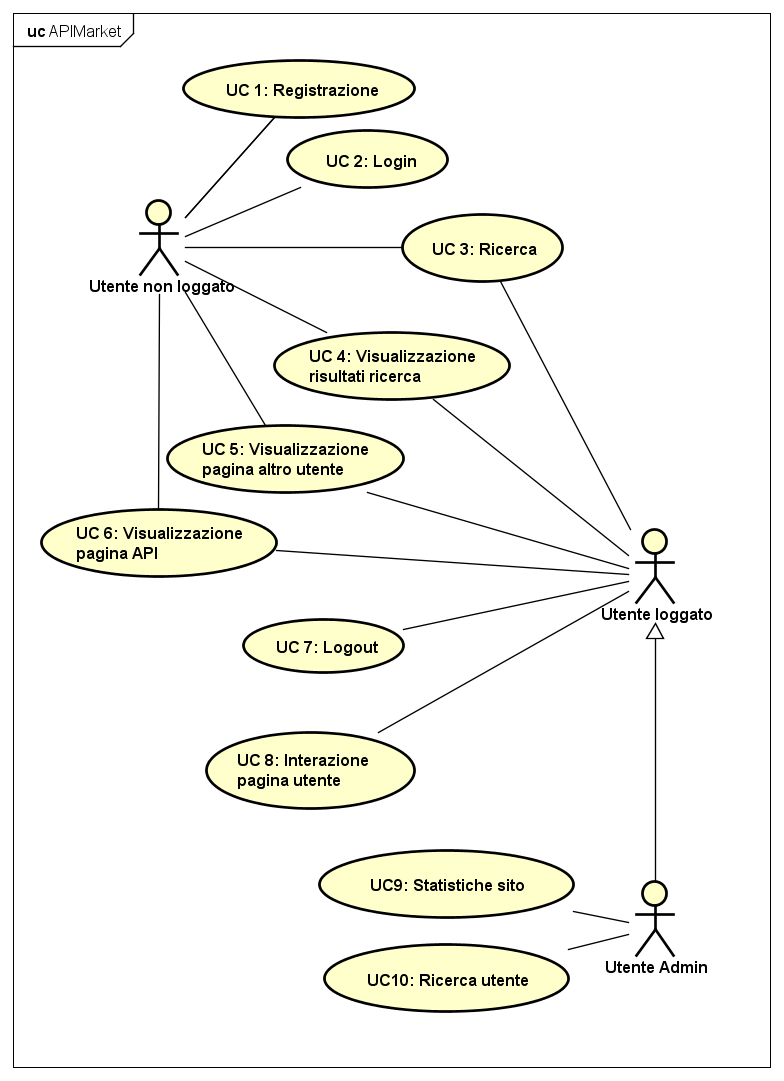
\includegraphics[width=0.7\textwidth]{UseCase/APIMarket}
	\caption{Operazioni ad alto livello}
\end{figure}
\begin{itemize}
	\item \textbf{Attori:} Utente non autenticato
	\item \textbf{Scopo e descrizione:} La pagina presenta tutti i servizi che sono offerti a un utente non autenticato ovvero:
	\begin{itemize} 
		\item Viene offerta la possibilità di registrarsi al market; 
		\item Viene offerta la possibilità di identificarsi se già in possesso di un account all'interno del market;
		\item Viene offerta la possibilità di consultare, solo a scopo informativo, le API all'interno del market (per poter caricare le proprie API, o acquistare APIKey è necessario accere con il proprio account); 
		\item Viene offerta la possibilità di consultare le statistiche riferite agli utenti all'interno del market;
	\end{itemize}
	\item \textbf{Precondizione:} Il sistema viene avviato da un utente esterno
	\item \textbf{Postcondizione:} Il sistema offre tutti servizi che un utente non autenticato può usufruire
\end{itemize}
\subsection{Caso d'uso UC1: Registrazione}
\begin{figure}[ht]
	\centering
	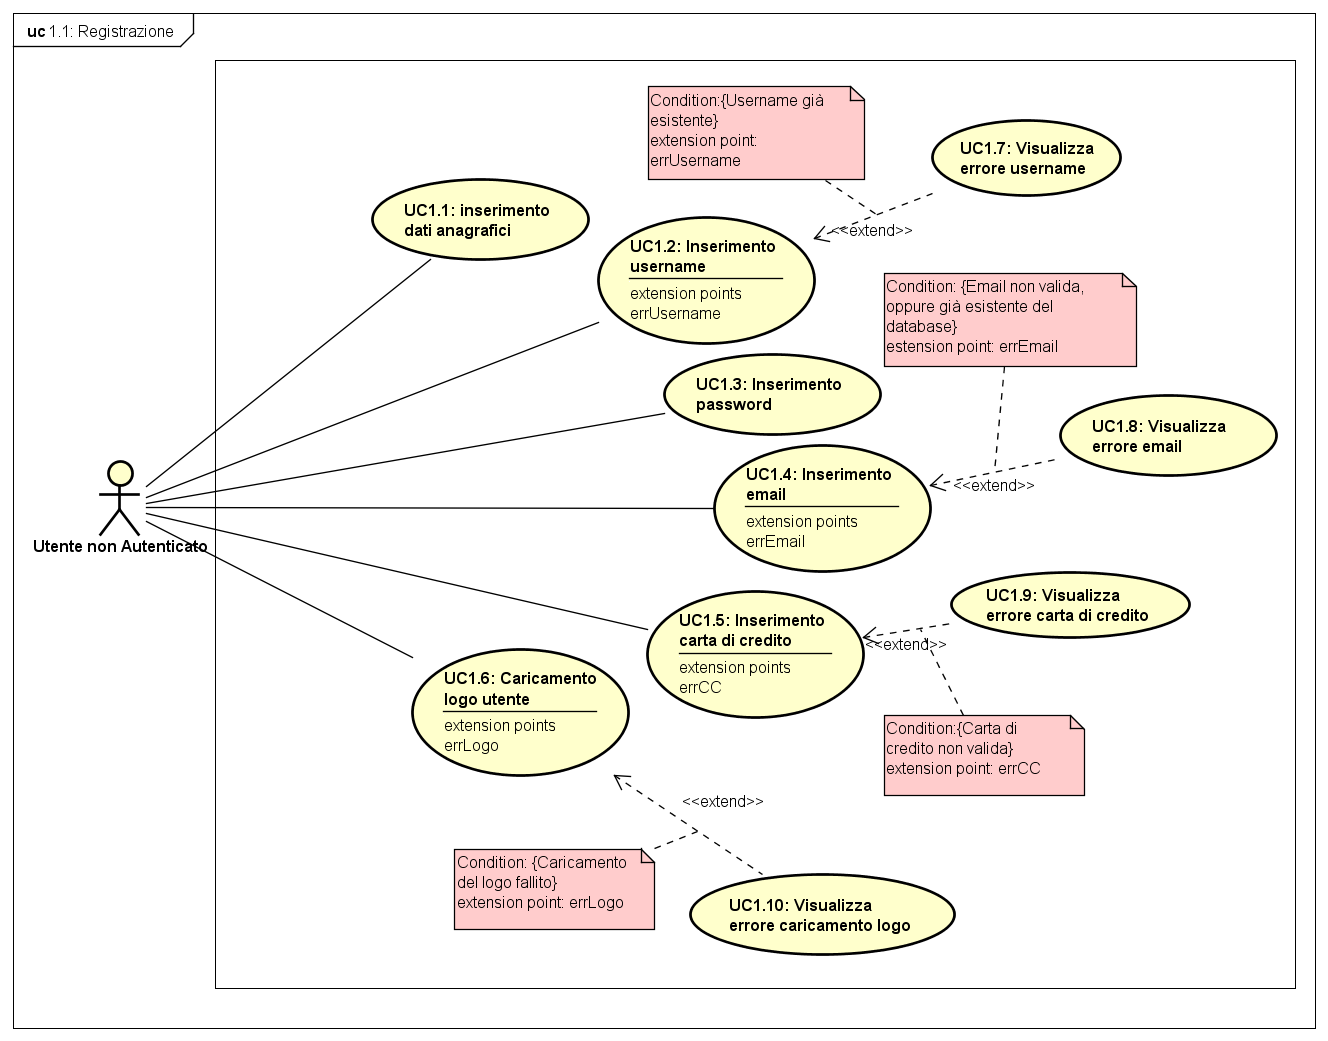
\includegraphics[width=0.7\textwidth]{UseCase/Registrazione}
	\caption{Registrazione}
\end{figure}
\begin{itemize}
	\item \textbf{Attori: Utente non autenticato}
	\item \textbf{Scopo e descrizione:} L'utente non i possesso di uno username e una password inserisce i suoi dati anagrafici da associare al nuovo username, gli verrà chiesta anche una password che dovrà utilizzare ogni qual volta debba effettare l'accesso;
	\item \textbf{Scenari alternativi:} Scenari alternativi: L'inserimento viene annullato per i seguenti motivi:
	\begin{itemize}
		\item username già esistente;
		\item password non soddisfa i criteri esposti. In tal caso viene richiesto all'utente di ripetere l'operazione.
	\end{itemize}
	\item \textbf{Precondizione:} Il sistema attende l'inserimento dei dati richiesti;
	\item \textbf{Postcondizione:} Il sistema si salva le informazione date dall'utente.
\end{itemize}
\subsection{Caso d'uso UC1.1: Inserimento dai anagrafici}
\begin{figure}[ht]
	\centering
	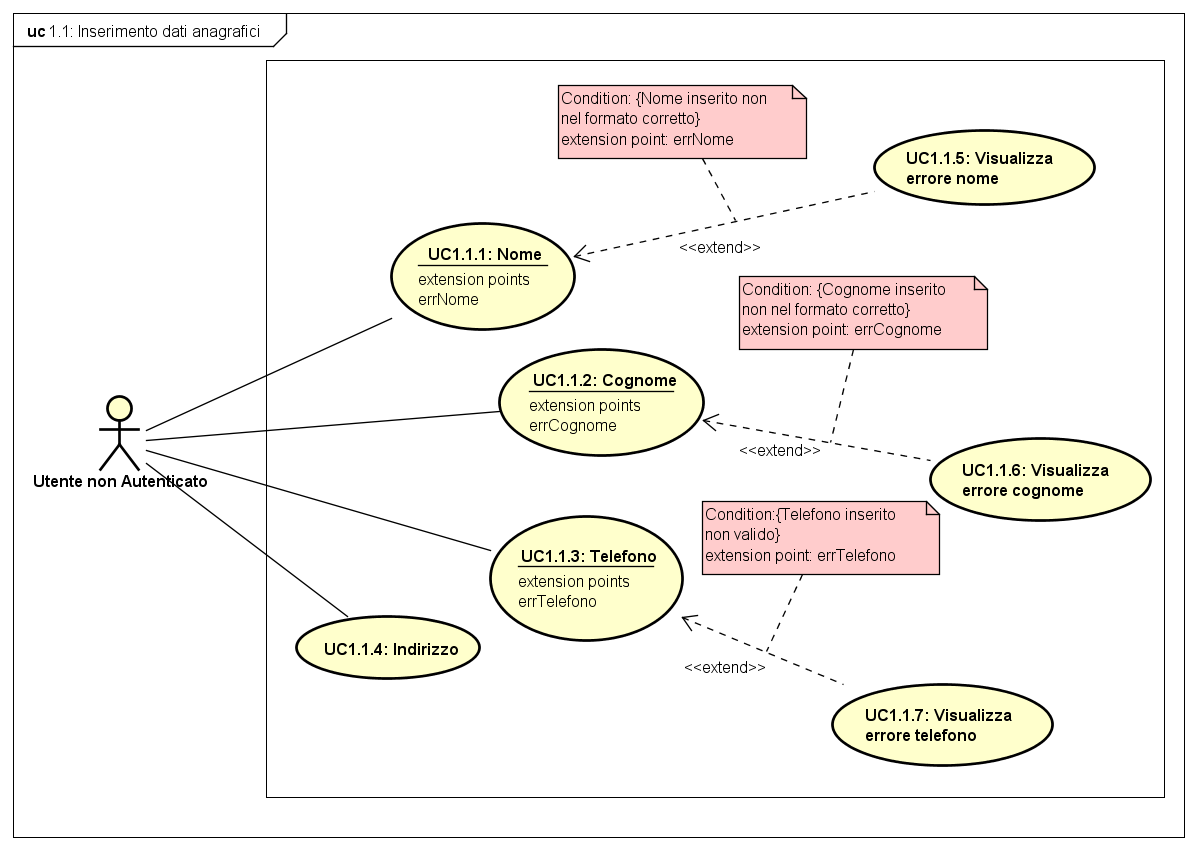
\includegraphics[width=0.7\textwidth]{UseCase/InserimentoDatiAnagrafici}
	\caption{Inserimento dati anagrafici}
\end{figure}
\begin{itemize}
	\item \textbf{Attori:} Utente non autenticato;
	\item \textbf{Scopo e descrizione:} L'utente non ancora autenticato inserisce i propri dati anagrafici (nome, cognome, nazionalità);
	\item \textbf{Precondizione:} Il sistema attende l'inserimento dei dati richiesti;
	\item \textbf{Postcondizione:} Il sistema salva le informazione date dall'utente.
\end{itemize}
\subsection{Caso d'uso UC1.1.1: Inserimento del nome}
\begin{itemize}
	\item \textbf{Attori:} Utente non autenticato; 
	\item \textbf{Scopo e descrizione:} L'utente deve inserire il suo nome;
	\item \textbf{Scenario alternativo:} Il nome inserito dall'utente non è conforme al formato richiesto;
	\item \textbf{Precondizione:} Il sistema attende l'inserimento del nome da parte dell'utente;
	\item \textbf{Postcondizione:} Il sistema inserisce nel DB il nome dell'utente.
\end{itemize}
\subsection{Caso d'uso UC1.1.2: Inserimento del cognome}
\begin{itemize}
	\item \textbf{Attori:} Utente non autenticato;
	\item \textbf{Scopo e descrizione:} L'utente deve inserire il suo nome;
	\item \textbf{Scenario alternativo:} Il nome inserito dall'utente non è conforme al formato richiesto;
	\item \textbf{Precondizione:} Il sistema attende l'inserimento del nome da parte dell'utente;
	\item \textbf{Postcondizione:} Il sistema inserisce nel DB il nome dell'utente.
\end{itemize}
\subsection{Caso d'uso UC1.1.3: Inserimento del telefono}
\begin{itemize}
	\item \textbf{Attori:} Utente non autenticato;
	\item \textbf{Scopo e descrizione:} L'utente deve inserire il suo numero di telefono;
	\item \textbf{Scenario alternativo:} Il numero di telefono inserito dall'utente non è valido;
	\item \textbf{Precondizione:} Il sistema attende l'inserimento del numero di telefono da parte dell'utente;
	\item \textbf{Postcondizione:} Il sistema inserisce nel DB il numero di telefono dell'utente.
\end{itemize}
\subsection{Caso d'uso UC1.1.4: Inserimento paese}
\begin{itemize}
	\item \textbf{Attori:} Utente non autenticato;
	\item \textbf{Scopo e descrizione:} L'utente deve inserire la nazionalità di appartenenza;
	\item \textbf{Scenario alternativo:} La nazionalità espressa dall'utente non esiste;
	\item \textbf{Precondizione:} Il sistema attende che l'utente scelga la nazionalità;
	\item \textbf{Postcondizione: }Il sistema inserisce nel DB il numero di telefono dell'utente.
\end{itemize}
\subsection{Caso d'uso UC1.2: Inserimento nome utente}
\begin{itemize}
	\item \textbf{Attori: }Utente non autenticato;
	\item \textbf{Scopo e descrizione: }L'utente inserisce lo username che gli servirà ad identificarsi nel sistema nel futuro;
	\item \textbf{Scenario alternativo: }Il sistema rifiuta lo username dato in quanto già presente nel DB, in tal caso viene chiesto di inserire all'utente un diverso username;
	\item \textbf{Precondizione: }Il sistema rimane in attesa dell'inserimento dello username;
	\item \textbf{Postcondizione: }Il sistema associa allo username i data anagrafici inseriti in precedenza e inserisce lo username nel DB degli utenti.
\end{itemize}
\subsection{Caso d'uso UC1.3: Inserimento password (Registrazione)}
\begin{figure}[H]
	\centering
	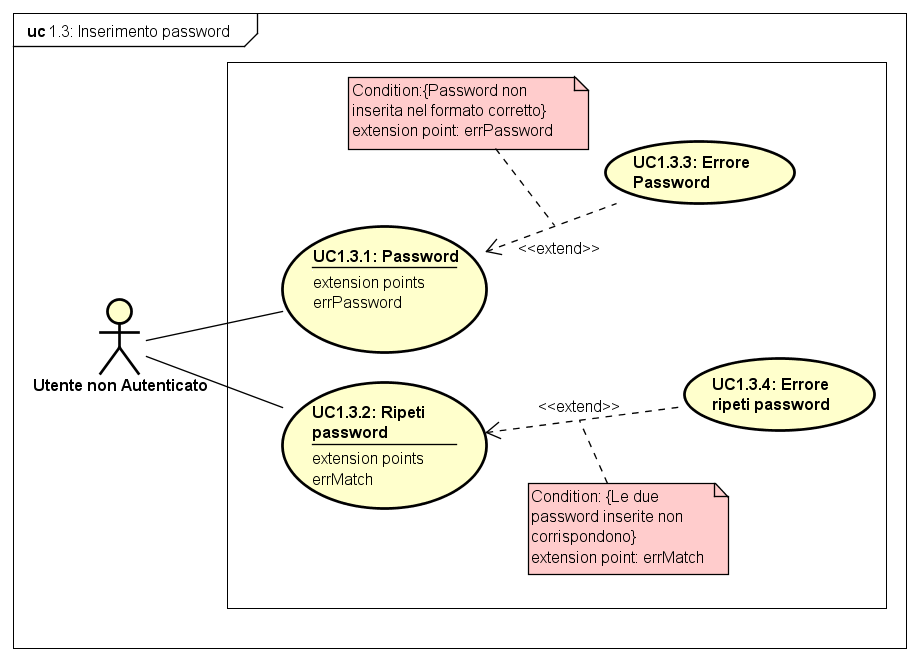
\includegraphics[width=0.7\textwidth]{UseCase/InserimentoPassword}
	\caption{Inserimento password (Registrazione)}
\end{figure}
\begin{itemize}
	\item \textbf{Attori: }Utente non autenticato;
	\item \textbf{Scopo e descrizione: } L'utente non autenticato inserisce una password che gli servirà come chiave di sicurezza per identificarsi nel sistema. La password richiesta, per poter essere accettata deve soddisfare i seguenti requisiti: 
	\begin{itemize}
		\item Deve essere lunga almeno 8 caratteri; 
		\item Deve contenere almeno 1 carattere maiuscolo; 
		\item Deve contere almeno 1 carattere minuscolo;
	\end{itemize}
	\item \textbf{Scenario alternativo: }La password inserita dall'utente non è conforme alle richieste, perciò il sistema chiede all'utente di inserire una nuova password che sia conforme;
	\item \textbf{Precondizione: }Il sistema attende che l'utente inserisca la password da associare al suo username;
	\item \textbf{Postcondizione: }Il sistema accetta la password inserita dall'utente e la associa allo username nel DB corrispondente.
\end{itemize}
\subsection{Caso d'uso UC1.4: Inserimento email)}
\begin{itemize}
	\item \textbf{Attori: }Utente non autenticato;
	\item \textbf{Scopo e descrizione: }Nel fututro nel caso in cui l'utente si fosse dimenticato la password, è necessario che il sistema abbia a disposizione un'email alla quale fare affidamento a cui poter mandare la password per poter far accedere l'utente;
	\item \textbf{Scenario alternativo: }L'email inserita non è nel formato valido, o esiste già nel database, quindi il sistema chiede all'utente di inserire un'altra email valida;
	\item \textbf{Precondizione: }Il sistema attende una email dall'utente;
	\item \textbf{Postcondizione: }Il sistema riceve una email che assocerà allo user name dell'utente.
\end{itemize}
\subsection{Caso d'uso UC1.5: Inserimento carta di credito}
\begin{itemize}
	\item \textbf{Attori: }Utente non autenticato;
	\item \textbf{Scopo e descrizione: }L'utente deve dispore di un metodo di una carta di credito valida che gli permetta di effettuare acquisti all'interno del market;
	\item \textbf{Scenario alternativo: }La carta di credito non è valida perciò viene segnalato errore e viene chiesto all'utente di inserirne uno diversa;
	\item \textbf{Precondizione: }Il sistema attende che l'utente inserisca una carta di credito valida;
	\item \textbf{Postcondizione: }Il sistema valida la carta di credito inserita dall'utente e la associa al suo account.
\end{itemize}
\subsection{Caso d'uso UC2: Login}
\begin{figure}[H]
	\centering
	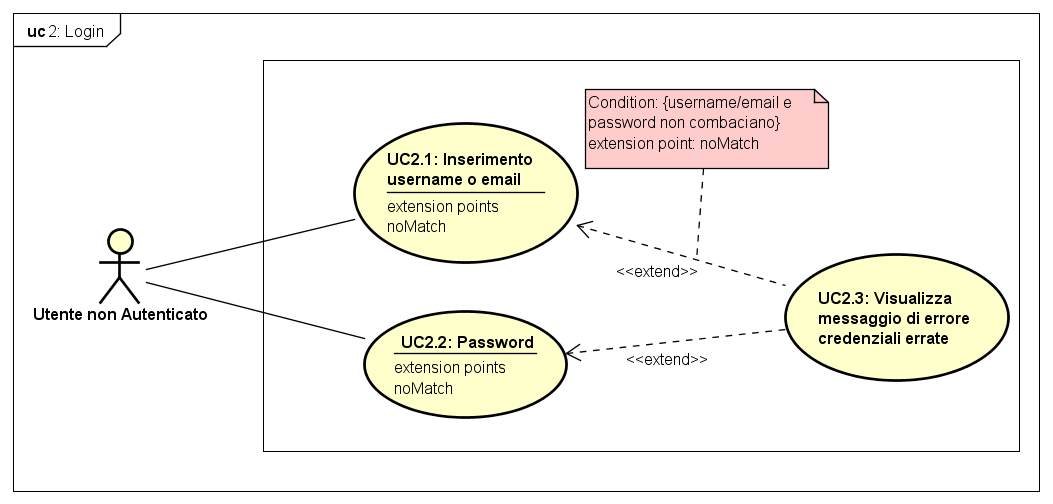
\includegraphics[width=0.7\textwidth]{UseCase/Login}
	\caption{Login}
\end{figure}
\begin{itemize}
	\item \textbf{Attori:} Utente non autenticato;
	\item \textbf{Scopo e descrizione:} L'utente che possiede già uno username e una password vuole effettuare un accesso;
	\item \textbf{Scenario alternativo: }Il sistema rifiuta l'accesso all'utente a causa di un errato inserimento di username o di password;
	\item \textbf{Precondizione: }Il sistema attende che l'utente inserisca i suoi dati identificativi;
	\item \textbf{Postcondizione: Il sistema ha accettato i dati e manda l'utente alla sua bacheca personale}.
\end{itemize}
\subsection{Caso d'uso UC2.1: Inserimento username o email}
\begin{itemize}
	\item \textbf{Attori: }Utente non autenticato;
	\item \textbf{Scopo e descrizione: }Viene chiesto all'utente di inserire il suo username o la sua email per poter essere identificato;
	\item \textbf{Scenario alternativo: }Lo username o l'email non esistono all'interno del DB;
	\item \textbf{Precondizione: }Il sistema attende l'inserimento dello username o dell'email da parte dell'utente;
	\item \textbf{Postcondizione: }Il sistema ha riconosciuto l'utente e attende l'inserimento della password per validare l'accesso.
\end{itemize}
\subsection{Caso d'uso UC2.2: Password}
\begin{itemize}
	\item \textbf{Attori: }Utente non autenticato;
	\item \textbf{Scopo e descrizione: }Viene chiesto all'utente di inserire la password associata allo username (o alla relativa email);
	\item \textbf{Scenario alternativo: }La password inserita dall'utente non corrispende alla password associata allo username perciò viene rifiutato l'accesso;
	\item \textbf{Precondizione: }Il sistema attende l'inserimento della password da parte dell'utente;
	\item \textbf{Postcondizione: }Il sistema ha verificato che la password inserita dall'utente è corretta perciò logga l'utente.
\end{itemize}
\subsection{Caso d'uso UC2.3: Recupero password}
\begin{itemize}
	\item \textbf{Attori: }Utente non autenticato;
	\item \textbf{Scopo e descrizione: }Nel caso in cui l'utente si fosse dimenticato la password del suo profilo, il sistema offre un'assistenza di recupero password, ovvero invierà alla mail associata al profilo una nuova password temporanea da utilizzare per accedervi e modificarla nuovamente;
	\item \textbf{Precondizione: }Il sistema rimane in attesa della richiesta da parte dell'utente di recuperare la sua password;
	\item \textbf{Postcondizione: }L'utente ha a disposizione una password temporanea che gli permette di accedere al suo profilo e modificarla nuovamente.
\end{itemize}
\subsection{Caso d'uso UC3: Ricerca}
\begin{figure}[H]
	\centering
	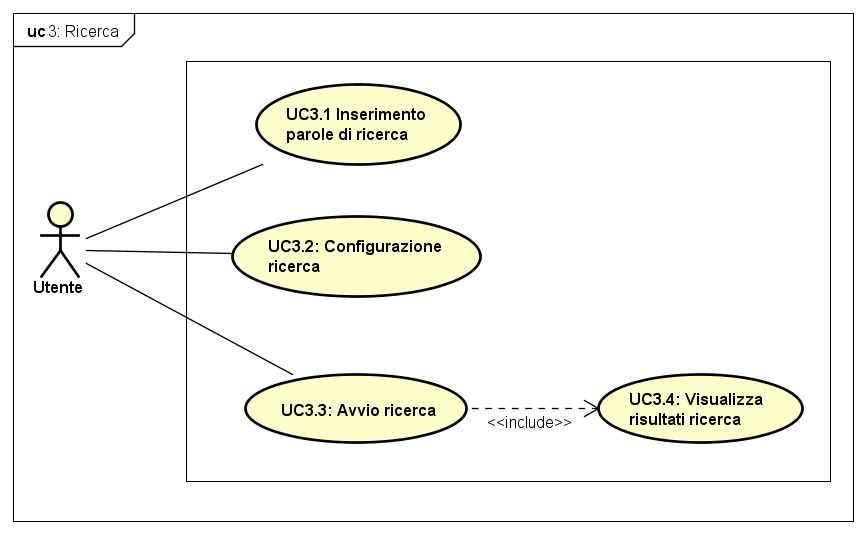
\includegraphics[width=0.7\textwidth]{UseCase/Ricerca}
	\caption{Ricerca}
\end{figure}
\begin{itemize}
	\item \textbf{Attori: }Utente non autenticato e Utente autenticato;
	\item \textbf{Scopo e descrizione: }L'utente ricerca nella barra di ricerca il nome di un microservizio e clicca il bottone di conferma;
	\item \textbf{Precondizione: }Il sistema attende l'invio di una frase di ricerca;
	\item \textbf{Postcondizione: }Il sistema ha esaminato la frase di ricerca e restituisce una pagina di risultati della ricerca.
\end{itemize}
\subsection{Caso d'uso UC3.1: Inserimento parole di ricerca}
\begin{itemize}
	\item \textbf{Attori: }Utente non autenticato e Utente autenticato;
	\item \textbf{Scopo e descrizione: }L'utente scrive nella barra di ricerca la frase che vuole ricercare;
	\item \textbf{Precondizione: }Il sistema attende l'inserimento di una frase di ricerca;
	\item \textbf{Postcondizione: }L'utente ha terminato di inserire la frase di ricerca.
\end{itemize}
\subsection{Caso d'uso UC3.2: Configurazione ricerca}
\begin{figure}[H]
	\centering
	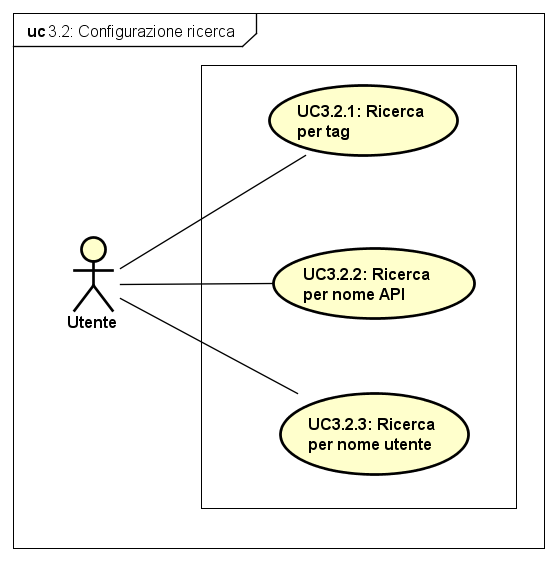
\includegraphics[width=0.7\textwidth]{UseCase/ConfigurazioneRicerca}
	\caption{Configurazione ricerca}
\end{figure}
\begin{itemize}
	\item \textbf{Attori: }Utente non autenticato e Utente autenticato;
	\item \textbf{Scopo e descrizione: }L'utente seleziona la modalità con cui vuole eseguire la ricerca;
	\item \textbf{Precondizione: }L'utente non ha ancora scelto nessun metodo di ricerca;
	\item \textbf{Postcondizione: }L'utente ha scelto un metodo di ricerca.
\end{itemize}
\subsection{Caso d'uso UC3.2.1: Ricerca per tag}
\begin{itemize}
	\item \textbf{Attori: }Utente non autenticato e Utente autenticato;
	\item \textbf{Scopo e descrizione: }L'utente sceglie di cercare all'interno di una categoria precisa di API;
	\item \textbf{Precondizione: }L'utente non ha ancora scelto la configurazione ricerca;
	\item \textbf{Postcondizione: }L'utente ha scelto il tag su cui effettuare la ricerca.
\end{itemize}
\subsection{Caso d'uso UC3.2.2: Ricerca per nome API}
\begin{itemize}
	\item \textbf{Attori: }Utente non autenticato e Utente autenticato;
	\item \textbf{Scopo e descrizione: }L'utente sceglie di cercare tra tutti i nomi dei microservizi del database;
	\item \textbf{Precondizione: }L'utente non ha ancora scelto la configurazione ricerca;
	\item \textbf{Postcondizione: }L'utente ha scelto la modalità di ricerca per nome API.
\end{itemize}
\subsection{Caso d'uso UC3.2.3: Ricerca per nome utente}
\begin{itemize}
	\item \textbf{Attori: }Utente non autenticato e Utente autenticato;
	\item \textbf{Scopo e descrizione: }L'utente sceglie di ricercare API tramite il nome utente dell'autore;
	\item \textbf{Precondizione: }L'utente non ha ancora scelto la configurazione ricerca;
	\item \textbf{Postcondizione: }L'utente ha scelto la modalità di ricerca per nome dell'autore.
\end{itemize}
\subsection{Caso d'uso UC3.3: Avvio ricerca}
\begin{itemize}
	\item \textbf{Attori: }Utente non autenticato e Utente autenticato;
	\item \textbf{Scopo e descrizione: }L'utente ha impostato la ricerca e preme il tasto per l'avvio della ricerca;
	\item \textbf{Precondizione: }L'utente ha finito di impostare la ricerca;
	\item \textbf{Postcondizione: }L'utente ha avviato la ricerca.
\end{itemize}
\end{document}